\documentclass[10pt]{article}
\usepackage{parskip}
\usepackage[utf8]{inputenc}
\usepackage[left=2.00cm, right=2.00cm, top=2.00cm, bottom=2.00cm]{geometry}
\usepackage[spanish]{babel}
\usepackage{graphicx,subfig}
\usepackage{fancyhdr}
\graphicspath{{Imagenes/}}
\usepackage{enumerate} 
\usepackage{multicol}
\usepackage{tabularx}
\begin{document}


\pagestyle{fancy}
\cfoot{}


%Cabeceras
\rhead{Multímetro.}
\lhead{}

%Portada
\begin{titlepage}
	\newgeometry{
		left=25mm,
		right=25mm,
		top=5mm,
		bottom=30mm,
		headheight = 0 mm
	}

	\begin{figure}[t]
		\subfloat{
\includegraphics[width=0.15\textwidth]{Logo_IPN}}
		\hspace{0.6\textwidth}
		\subfloat{
\includegraphics[width=0.22\textwidth]{LogoEsime}}
	\end{figure}

	\centering
	{\bfseries\Huge Instituto Politécnico Nacional. \par}
	\vspace{1cm}
	{\scshape\Large Ingeniería en Comunicaciones y Electrónica. \par}
	\vspace{0.3cm}
	{\scshape\Large Laboratorio de Electricidad y Magnetismo.  \par}
	\vspace{1cm}
	{\scshape\Huge El Universo de las Mediciones Eléctricas. \par}
	\vspace{1cm}
	{\itshape\Large Multímetro. \par}
	{\Large 2CM13\par}
	\vfill
	{\Large Autores: \par}
	{\Large Daniela Elizabeth Pérez Vargas. \par}
	{\Large Jesús Martinez Amac. \par}
	{\Large José Emilio Hernández Huerta. \par}
	{\Large Nataly Bejarano Garduño.\par}
	{\Large Uriel Grimaldi Díaz.  \par}
	\vfill
	{\Large Mayo 2023. \par}

\end{titlepage}

\tableofcontents
\newpage

\section{Resumen.}
En la presente práctica, se desarrolla el uso del multímetro con enfásis en las funciones de medición de resistencia, continuidad, vóltmetro (Corriente Directa y Corriente Alterna) y Amperímetro. 

\begin{multicols}{2}

\section{Objetivo.}

El alumno será capaz de describir las características y funcionamiento del multímetro así como manejar correctamente dicho instrumento para realizar mediciones de las 3 magnitudes eléctricas fundamentales (Resistencia, Potencial eléctrico y Corriente eléctrica).

\section{Introducción.}

La herramienta fundamental del técnico o ingeniero especializado en la manipulación de componentes electrónicos es el multímetro, dicha herramienta permite al profesional obtener mediciones de magnitudes eléctricas que le puedan resultar útiles,
estas magnitudes suelen ser , la resistencia eléctrica, el potencial eléctrico, la corriente eléctrica,frecuencia, inductancia, capacitancia además de otras utilidades como la continuidad y la prueba de diodos.

\section{Marco teórico.}



\section{Descripción de materiales.}

\begin{center}

	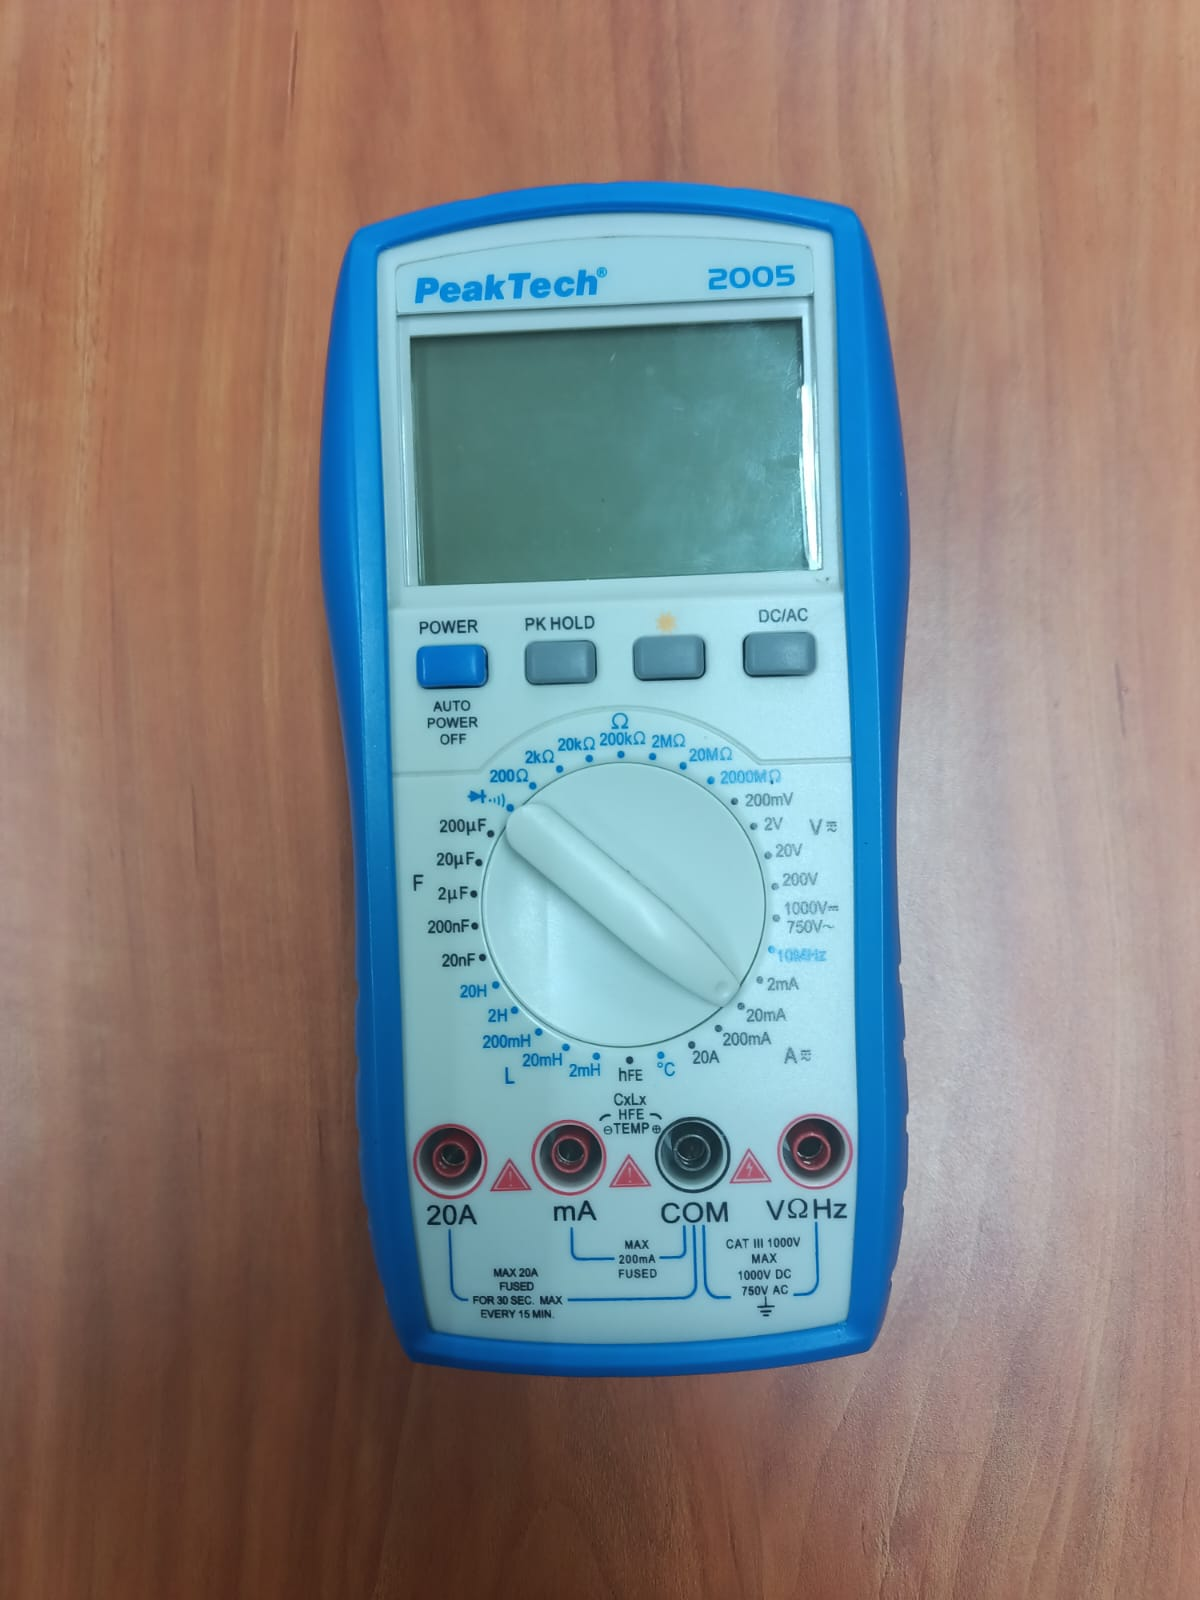
\includegraphics[scale = 0.1]{Imagenes/Material/MultiD.jpeg}\\
	Multímetro Digital.

	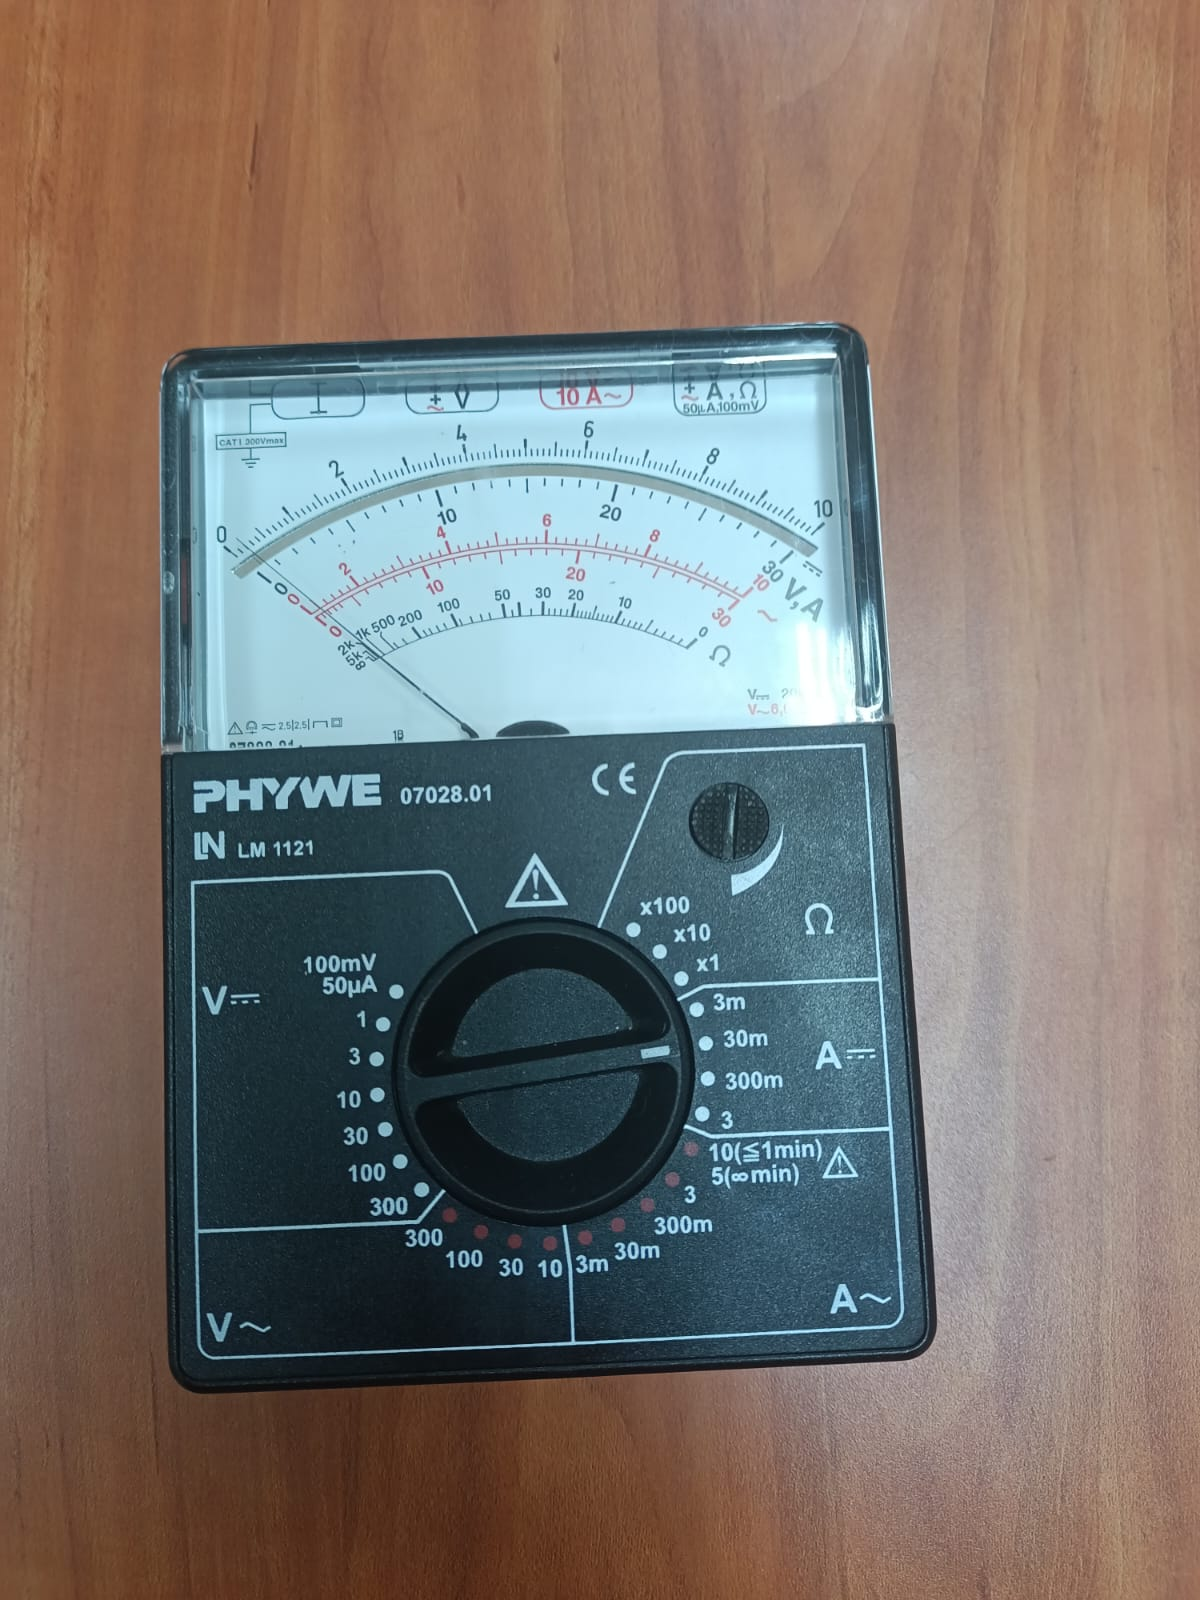
\includegraphics[scale = 0.1]{Imagenes/Material/MultiA.jpeg}\\
	Multímetro Analógico.

	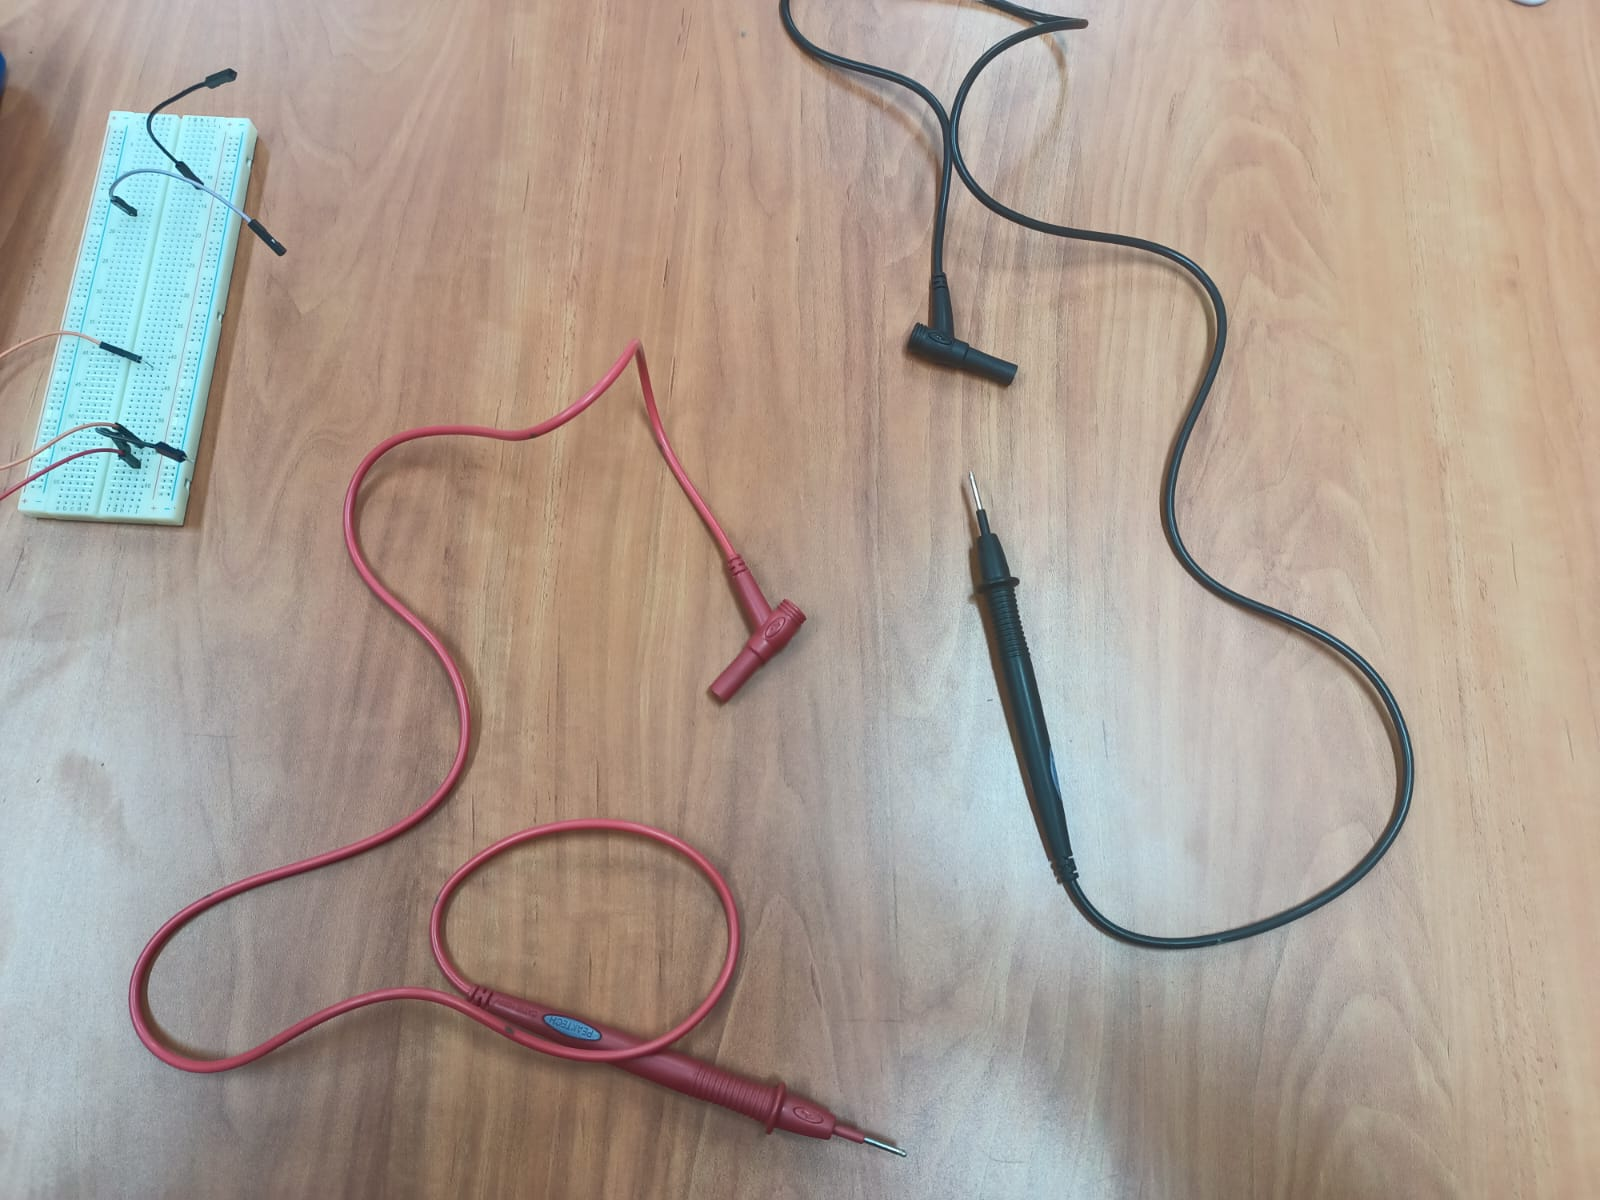
\includegraphics[scale = 0.1]{Imagenes/Material/Puntas.jpeg}\\
	Puntas para multímetro.

	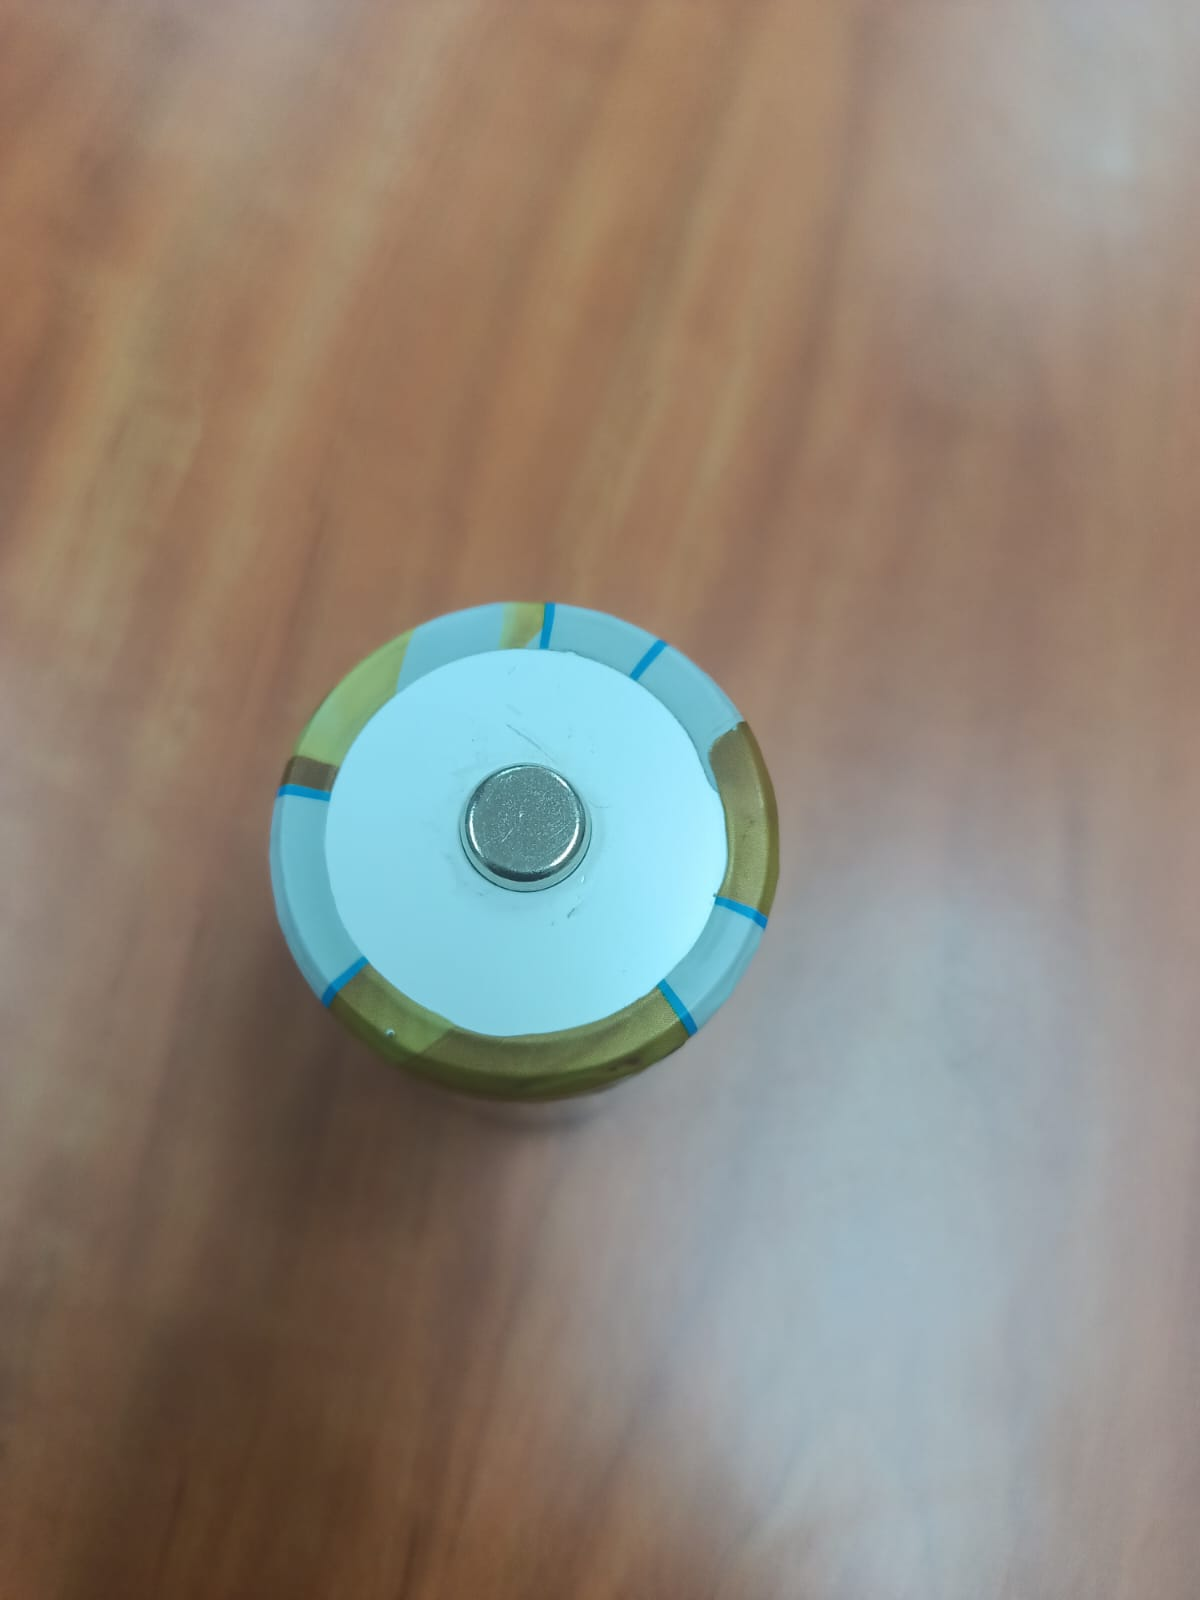
\includegraphics[scale = 0.1]{Imagenes/Material/PilaD.jpeg}\\
	Pila tipo "D" de 1.5 V.

	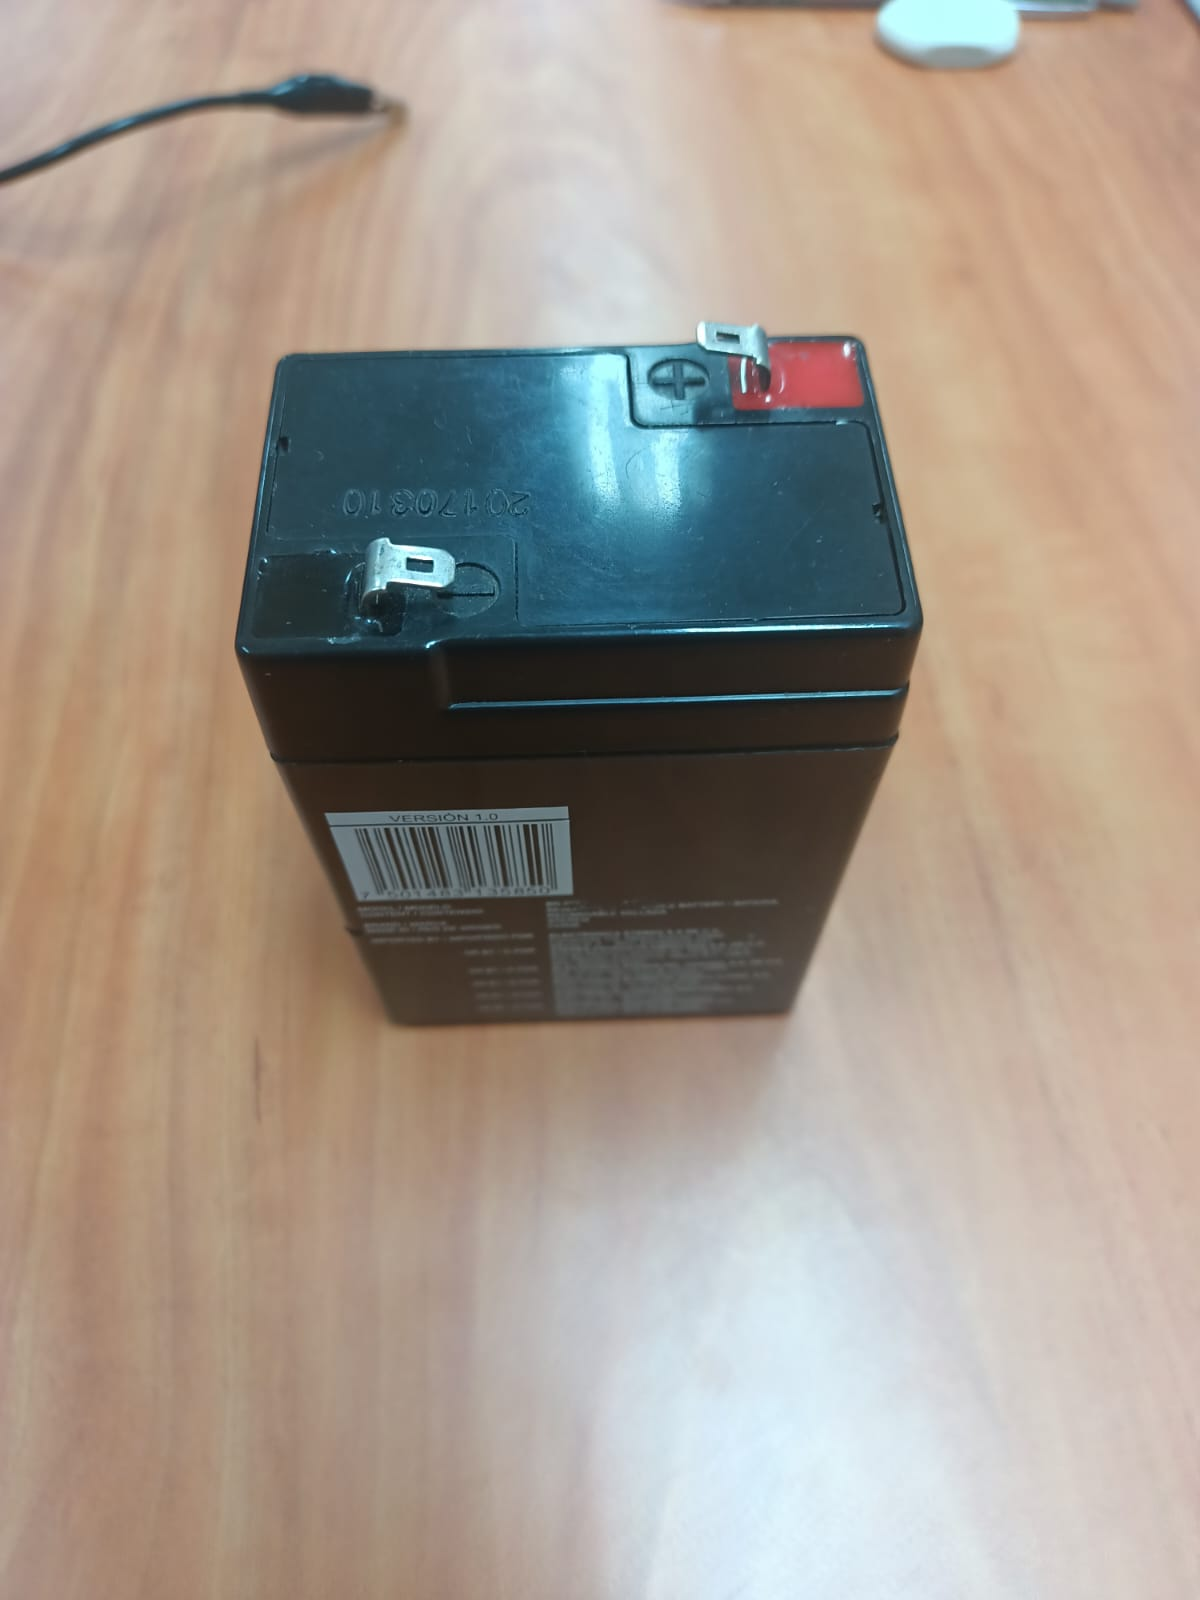
\includegraphics[scale = 0.1]{Imagenes/Material/PilaDes.jpeg}\\
	Pila de valor desconocido.

	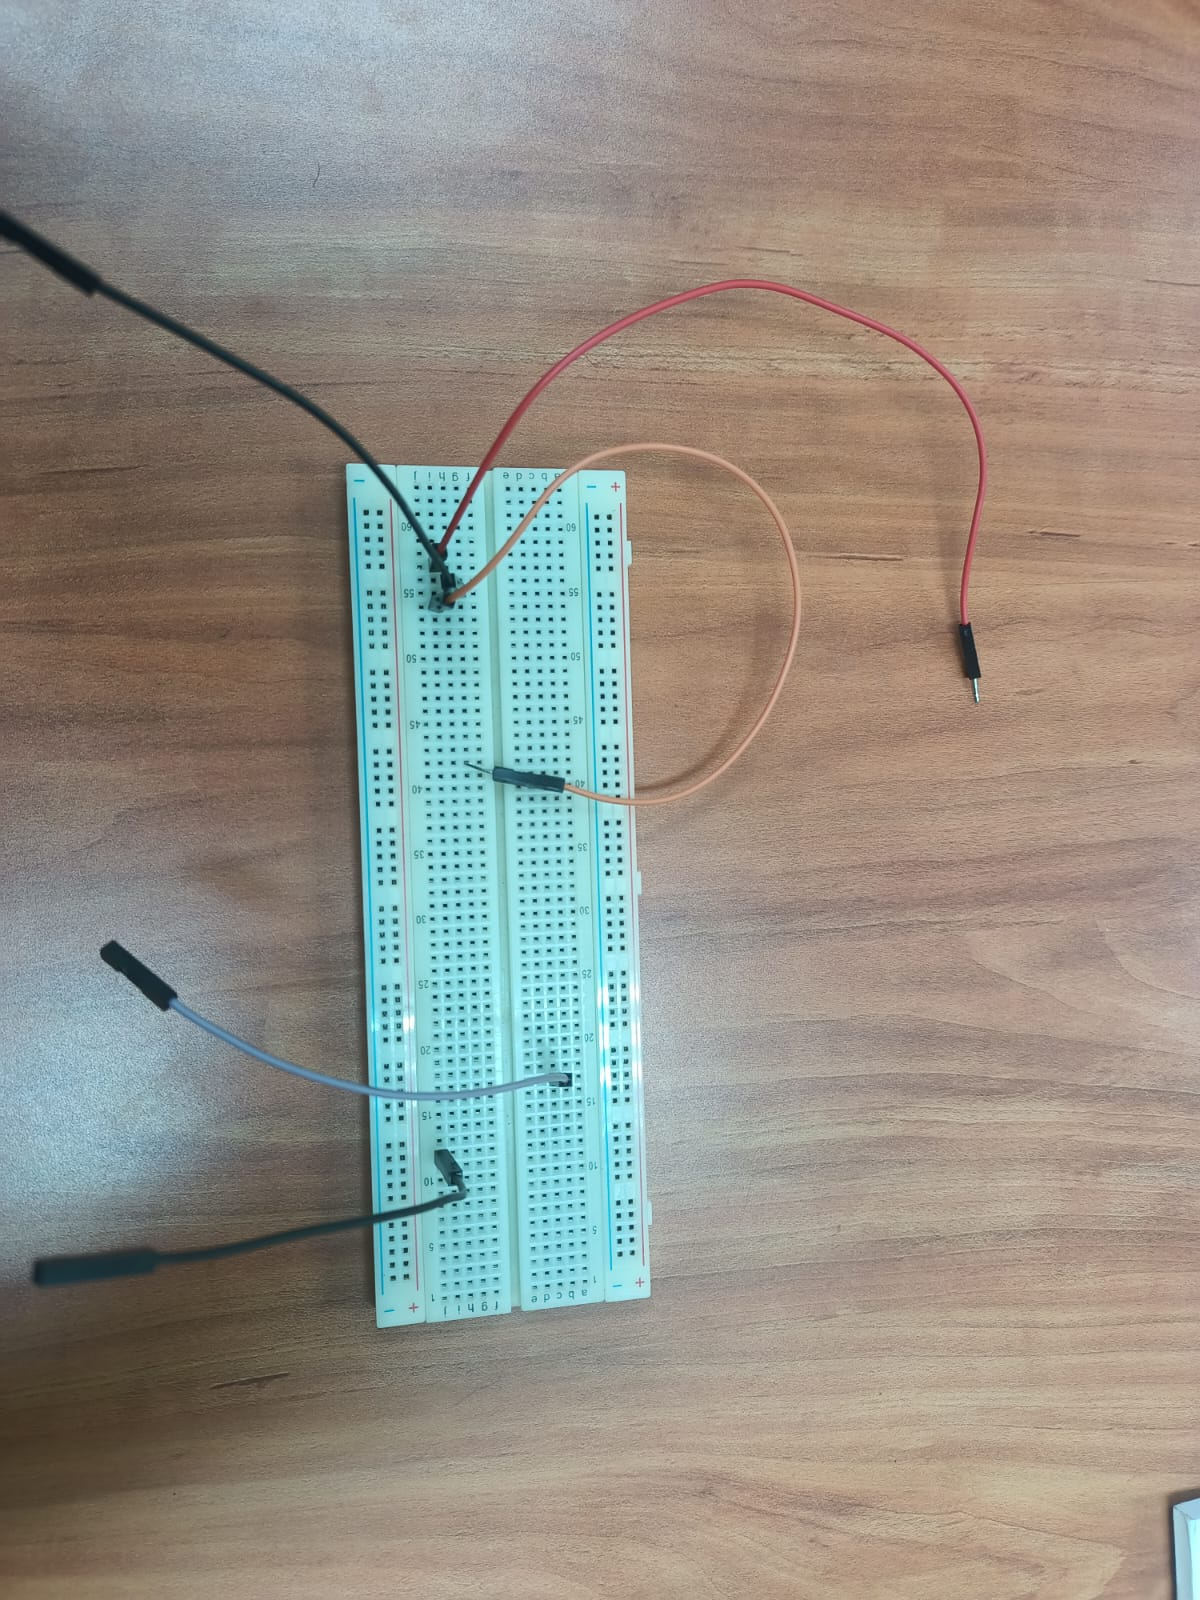
\includegraphics[scale = 0.1]{Imagenes/Material/Protoboard y jumper.jpeg}\\
	Protoboard y Jumpers.

	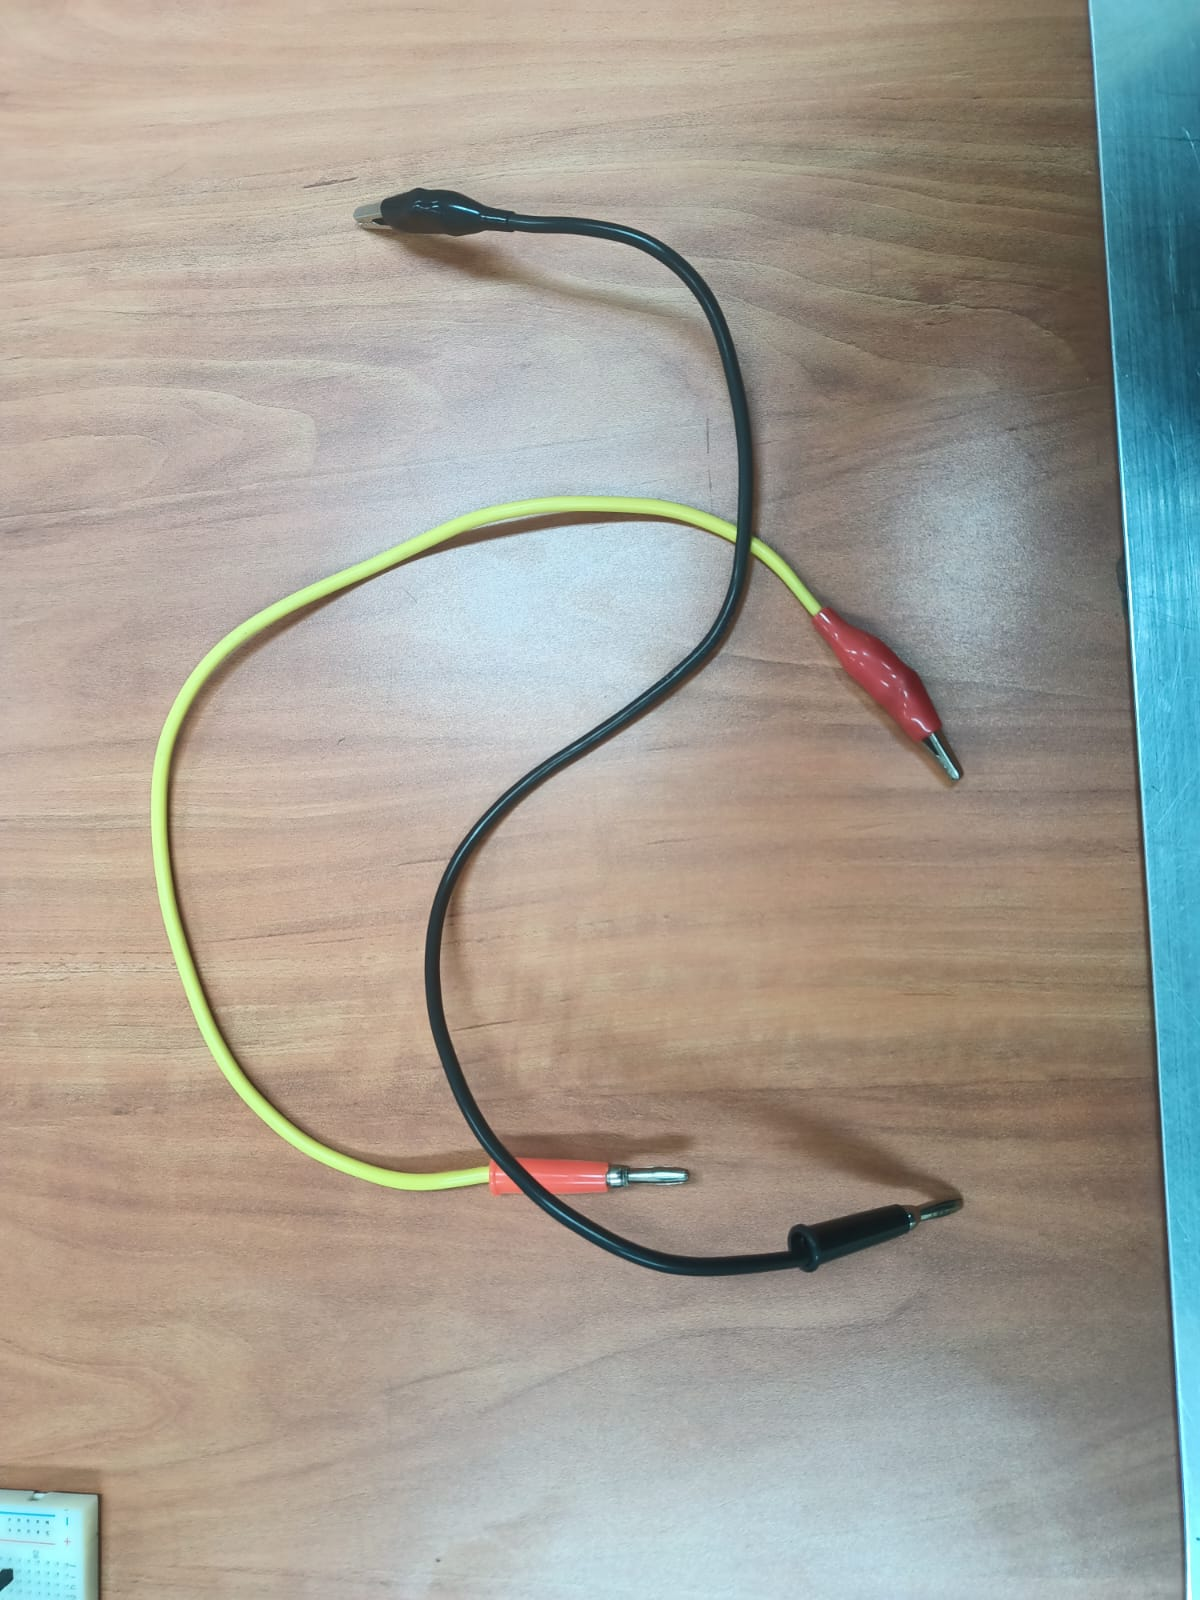
\includegraphics[scale = 0.1]{Imagenes/Material/Caimanban.jpeg}\\
	Cables <<Caimán-Banana>>.

	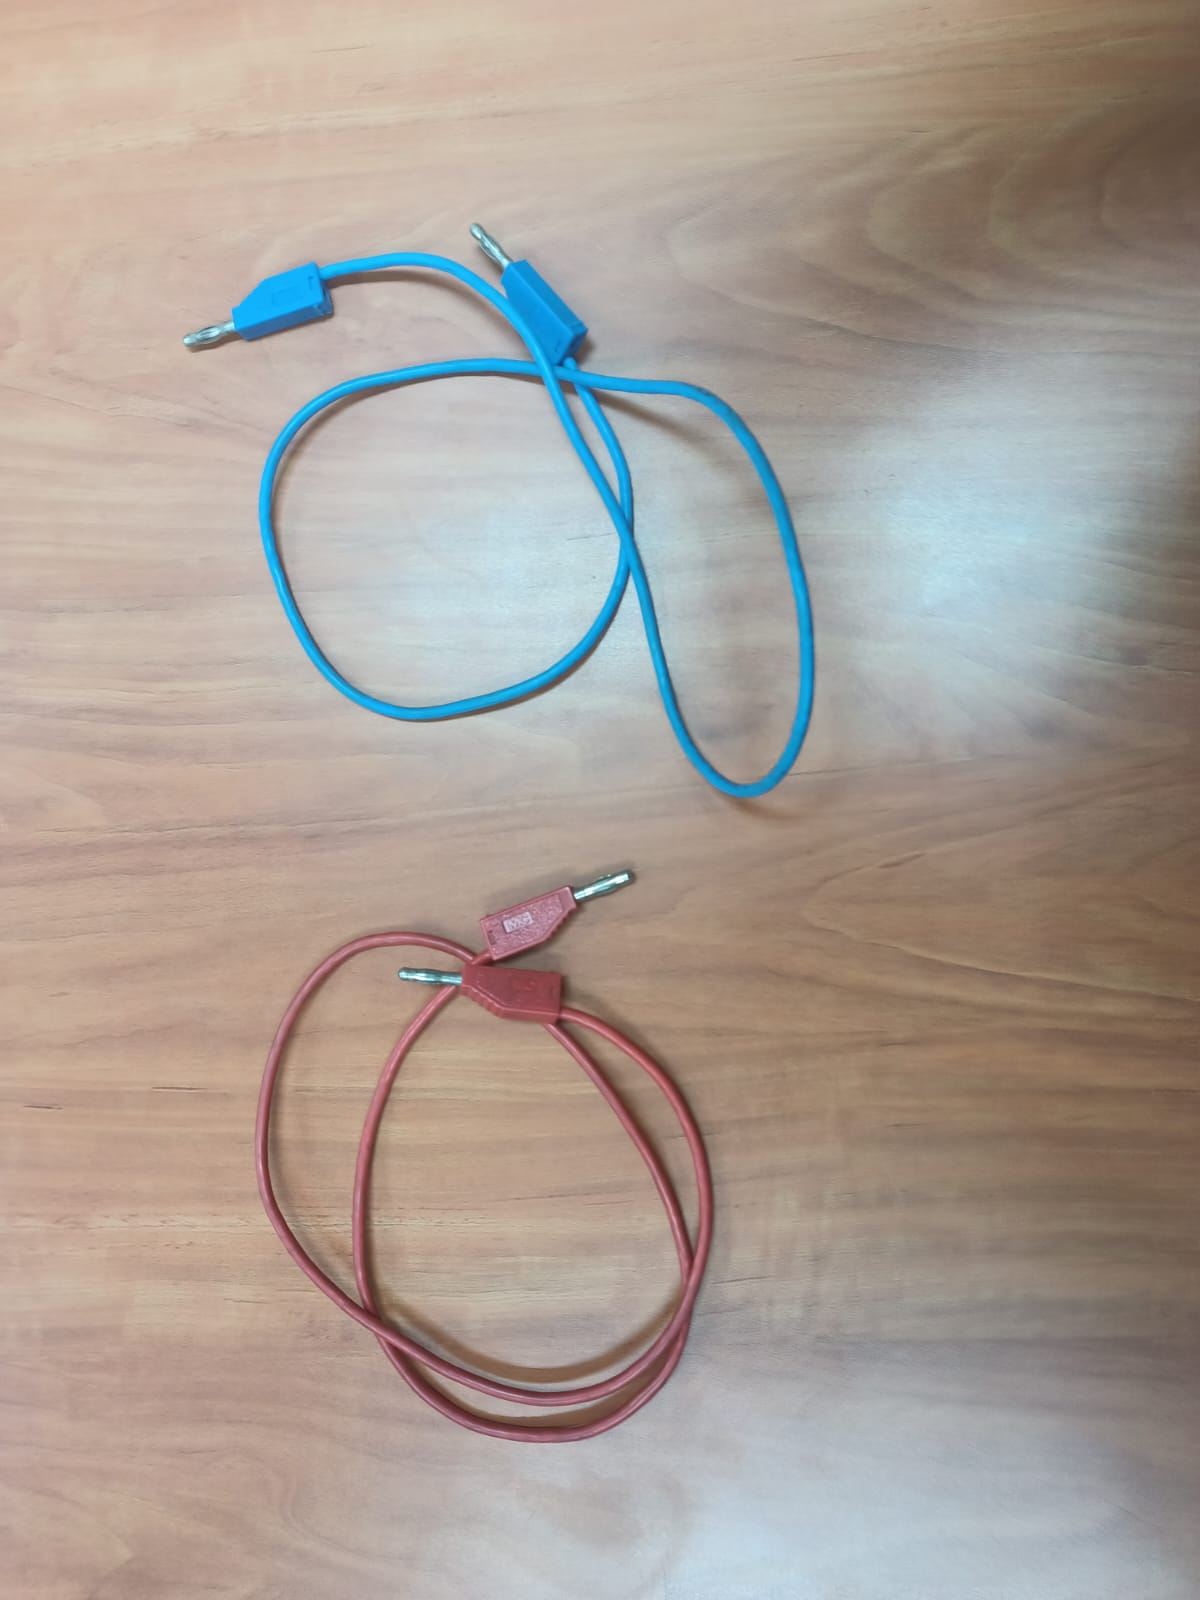
\includegraphics[scale = 0.1]{Imagenes/Material/banban.jpeg}\\
	Cables <<Banana-Banana>>.

	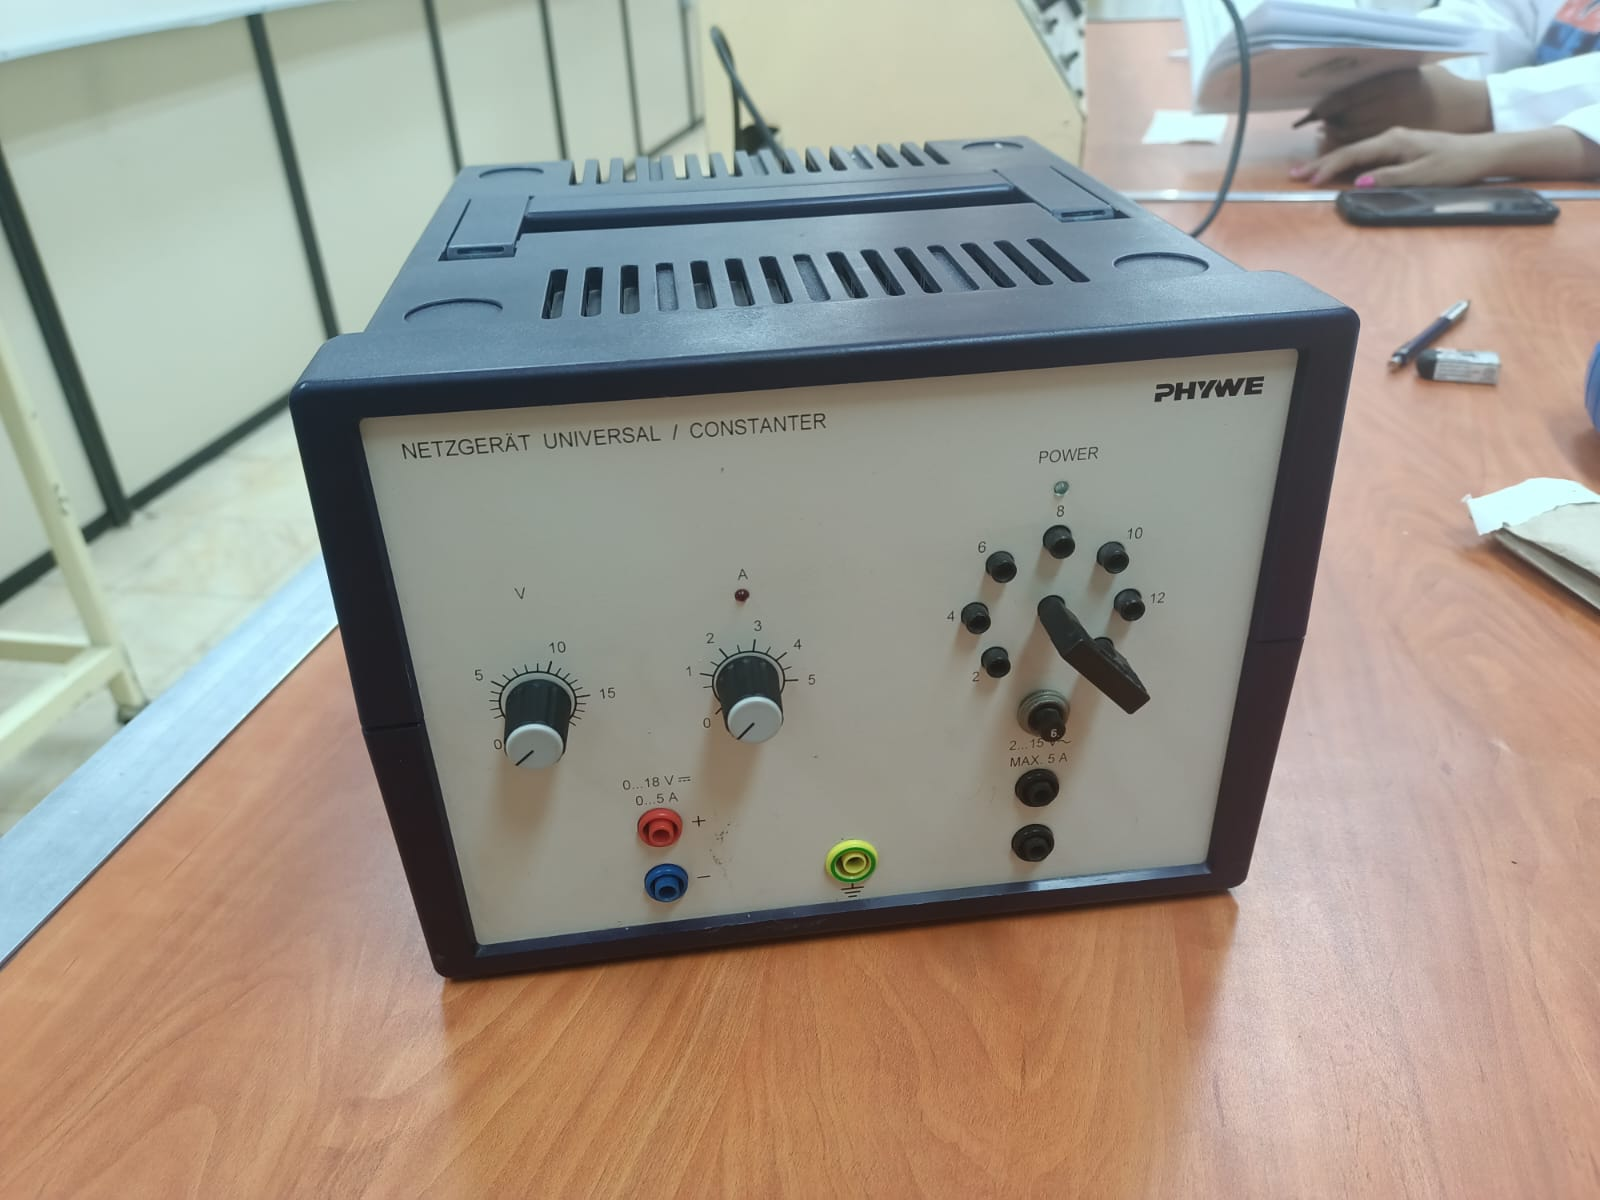
\includegraphics[scale = 0.1]{Imagenes/Material/FuenteVariable.jpeg}\\
	Fuente de alimentación regulada.

	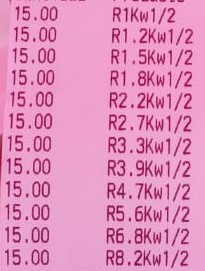
\includegraphics[scale = 1]{Imagenes/Material/Resistencias.jpeg}\\
	Resistencias de valores entre 1K$\Omega$ y 9K$\Omega$

\end{center}


\section{Desarrollo experimental.}

\subsection{Reconocimiento del multímetro.}

Tome el multímetro digital y reconozca lo siguiente:
\begin{enumerate}
	\item La marca y modelo del multímetro.
	\item Como encender el multímetro.
	\item Cuántas posiciones y cuáles son los rangos del multímetro para medir voltajes de Corriente Directa.
	\item Cuántas posiciones y cuáles son los rangos del multímetro para medir corrientes de Corriente Directa y Corriente Alterna.
	\item Cuántos y cuáles son los rangos del multímetro para medir resistencia.
	\item Otras funciones,interruptores y selectores.
\end{enumerate}

\subsection{Mediciones de resistencia(óhmetro).}

\begin{enumerate}
	\item Encienda el multimetro y coloque la perilla en Ohms.
	\item Anote los valores utilizando el código de colores para resistores.
	\item Mida los resistores y anote los valores obtenidos en una tabla.
	\item Compare el valor nominal con el valor medido.
\end{enumerate}

\subsection{Mediciones de continuidad.}

\begin{enumerate}
	\item Utilizando el medidor de continuidad o en la escala de resistencia más baja identifique como está constituida una protoboard.
	\item Elabore un diagrama según lo observado.
\end{enumerate}

\subsection{Mediciones de voltaje(vóltmetro).}

\begin{enumerate}
	\item Coloque la perilla del multímero en volts y ubique correctamente el selector de tipo de corriente en Corriente Directa.
	\item Mida el voltaje de las pilas y anote sus valores.
	\item Utilice la fuente regulada, ubique las salidas de corriente directa y realice tres mediciones diferentes respetando la polaridad.
\end{enumerate}

\subsection{Mediciones de voltaje de corriente alterna(vóltmetro).}

\begin{enumerate}
	\item Ubique un contacto como el mostrado en la siguiente imagen.\\
	\begin{center}
		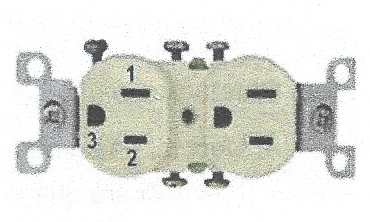
\includegraphics{Imagenes/Fotos/Contacto.png}
	\end{center}
	\item Mida el voltaje entre salidas y anote su valor.
	\item Identifique en el contacto cuál es la fase,el neutro y la tierra física.
\end{enumerate}

\subsection{Mediciones de intensidad de corriente continua(Amperímetro.)}
\begin{enumerate}
	\item Arme el siguiente circuito.\\
	\begin{center}
		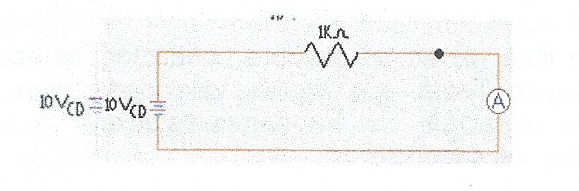
\includegraphics{Imagenes/Fotos/Circuito.png}
	\end{center}
	\item Seleccione una escala de medición adecuada y coloque el selector de Corriente Alterna y Corriente Directa en Corriente Directa.
	\item Mida la corriente en el circuito.
	\item Calcule el valor teórico de la corriente del circuito y compare con el valor medido.
\end{enumerate}

\section{Discusión de materiales .}


\section{Análisis y resultados.}

\subsection{Reconocimiento del multímetro.}
 

\subsection{Mediciones de resistencia(óhmetro).}

\begin{adjustbox}{width=\textwidth}
	\begin{tabular}{|c|c|c|c|c|}
		\hline
		Resistencia & Colores & Tolerancia & Valor nominal (ohms) & Valor medido (ohms) \\
		\hline
		1 & Café, verde, rojo, dorado & $\pm$ 5\% & 1.5 & 1.46 \\
		\hline
		2 & Rojo, azul, rojo, dorado & $\pm$ 5\% & 2.2 & 2.18 \\
		\hline
		3 & Naranja, naranja, naranja, dorado & $\pm$ 5\% & 3.3 & 3.28 \\
		\hline
		4 & Amarillo, violeta, rojo, dorado & $\pm$ 5\% & 4.7 & 4.75 \\
		\hline
		5 & Café, negro, negro, dorado & $\pm$ 5\% & 5.7 & 5.72 \\
		\hline
	\end{tabular}
\end{adjustbox}

\subsection{Mediciones de continuidad.}

\subsection{Mediciones de voltaje(vóltmetro).}
\begin{tabular}{ p{4cm} p{3cm} }
	\hline
	Pila 1 : & 0.82 volts \\
	\hline
	Pila 2 : & 5.8 volts \\
	\hline
\end{tabular}

\subsection{Mediciones de voltaje de corriente alterna(vóltmetro).}

\subsection{Mediciones de intensidad de corriente continua(Amperímetro.)}




\section{Conclusiones.}

\subsection*{Daniela Elizabeth Pérez Vargas.}

\subsection*{Jesús Martinez Amac.}
\subsection*{José Emilio Hernández Huerta.}
En esta practica con los diferentes tipos de medición que hicimos llegamos a diferentes conclusiones, la primera antes de la existencia de multímetros existían herramientas de medición como el voltímetro especializado en medir el potencial eléctrico, el amperímetro para medir el amperaje de los circuitos eléctricos, entre otros más. Con la llegada del multímetro todo esto se juntó ayudando a mejorar las mediciones con solo un aparato de medición. Al igual que me deja con dudas como: ¿Cómo funcionan?, ¿Qué hacen los automáticos para saber solos el rango de medidas?, etc. Otra de las cosas que puede medir el multímetro es la temperatura y la frecuencia, ambas generándome intriga por saber de la misma forma como funcionan. Yo solo espero las prácticas de electrónica para poder emplear los conocimientos adquiridos en esta practica en un ambiente un poco mas cercano a la realidad. 
\subsection*{Nataly Bejarano Garduño.}
\subsection*{Uriel Grimaldi Díaz.}

\end{multicols}
\newpage
\clearpage
\begin{thebibliography}{0}
	\bibitem{citekey}
\end{thebibliography}

\end{document}
